\graphicspath{{./figures/ux-ui/}}

\section{UX/UI}

\subsection{Flujo de Interacción del Usuario}

El flujo de interacción de Amazon Copilot está diseñado para proporcionar una experiencia de usuario intuitiva y eficiente. La aplicación presenta tres páginas principales que guían al usuario a través de su jornada de compra.

\subsubsection{Página Principal - Catálogo de Productos}

La página principal (\textit{Home}) sirve como punto de entrada a la aplicación, presentando un catálogo completo de productos con funcionalidades avanzadas de búsqueda y filtrado.

\begin{figure}[H]
    \centering
    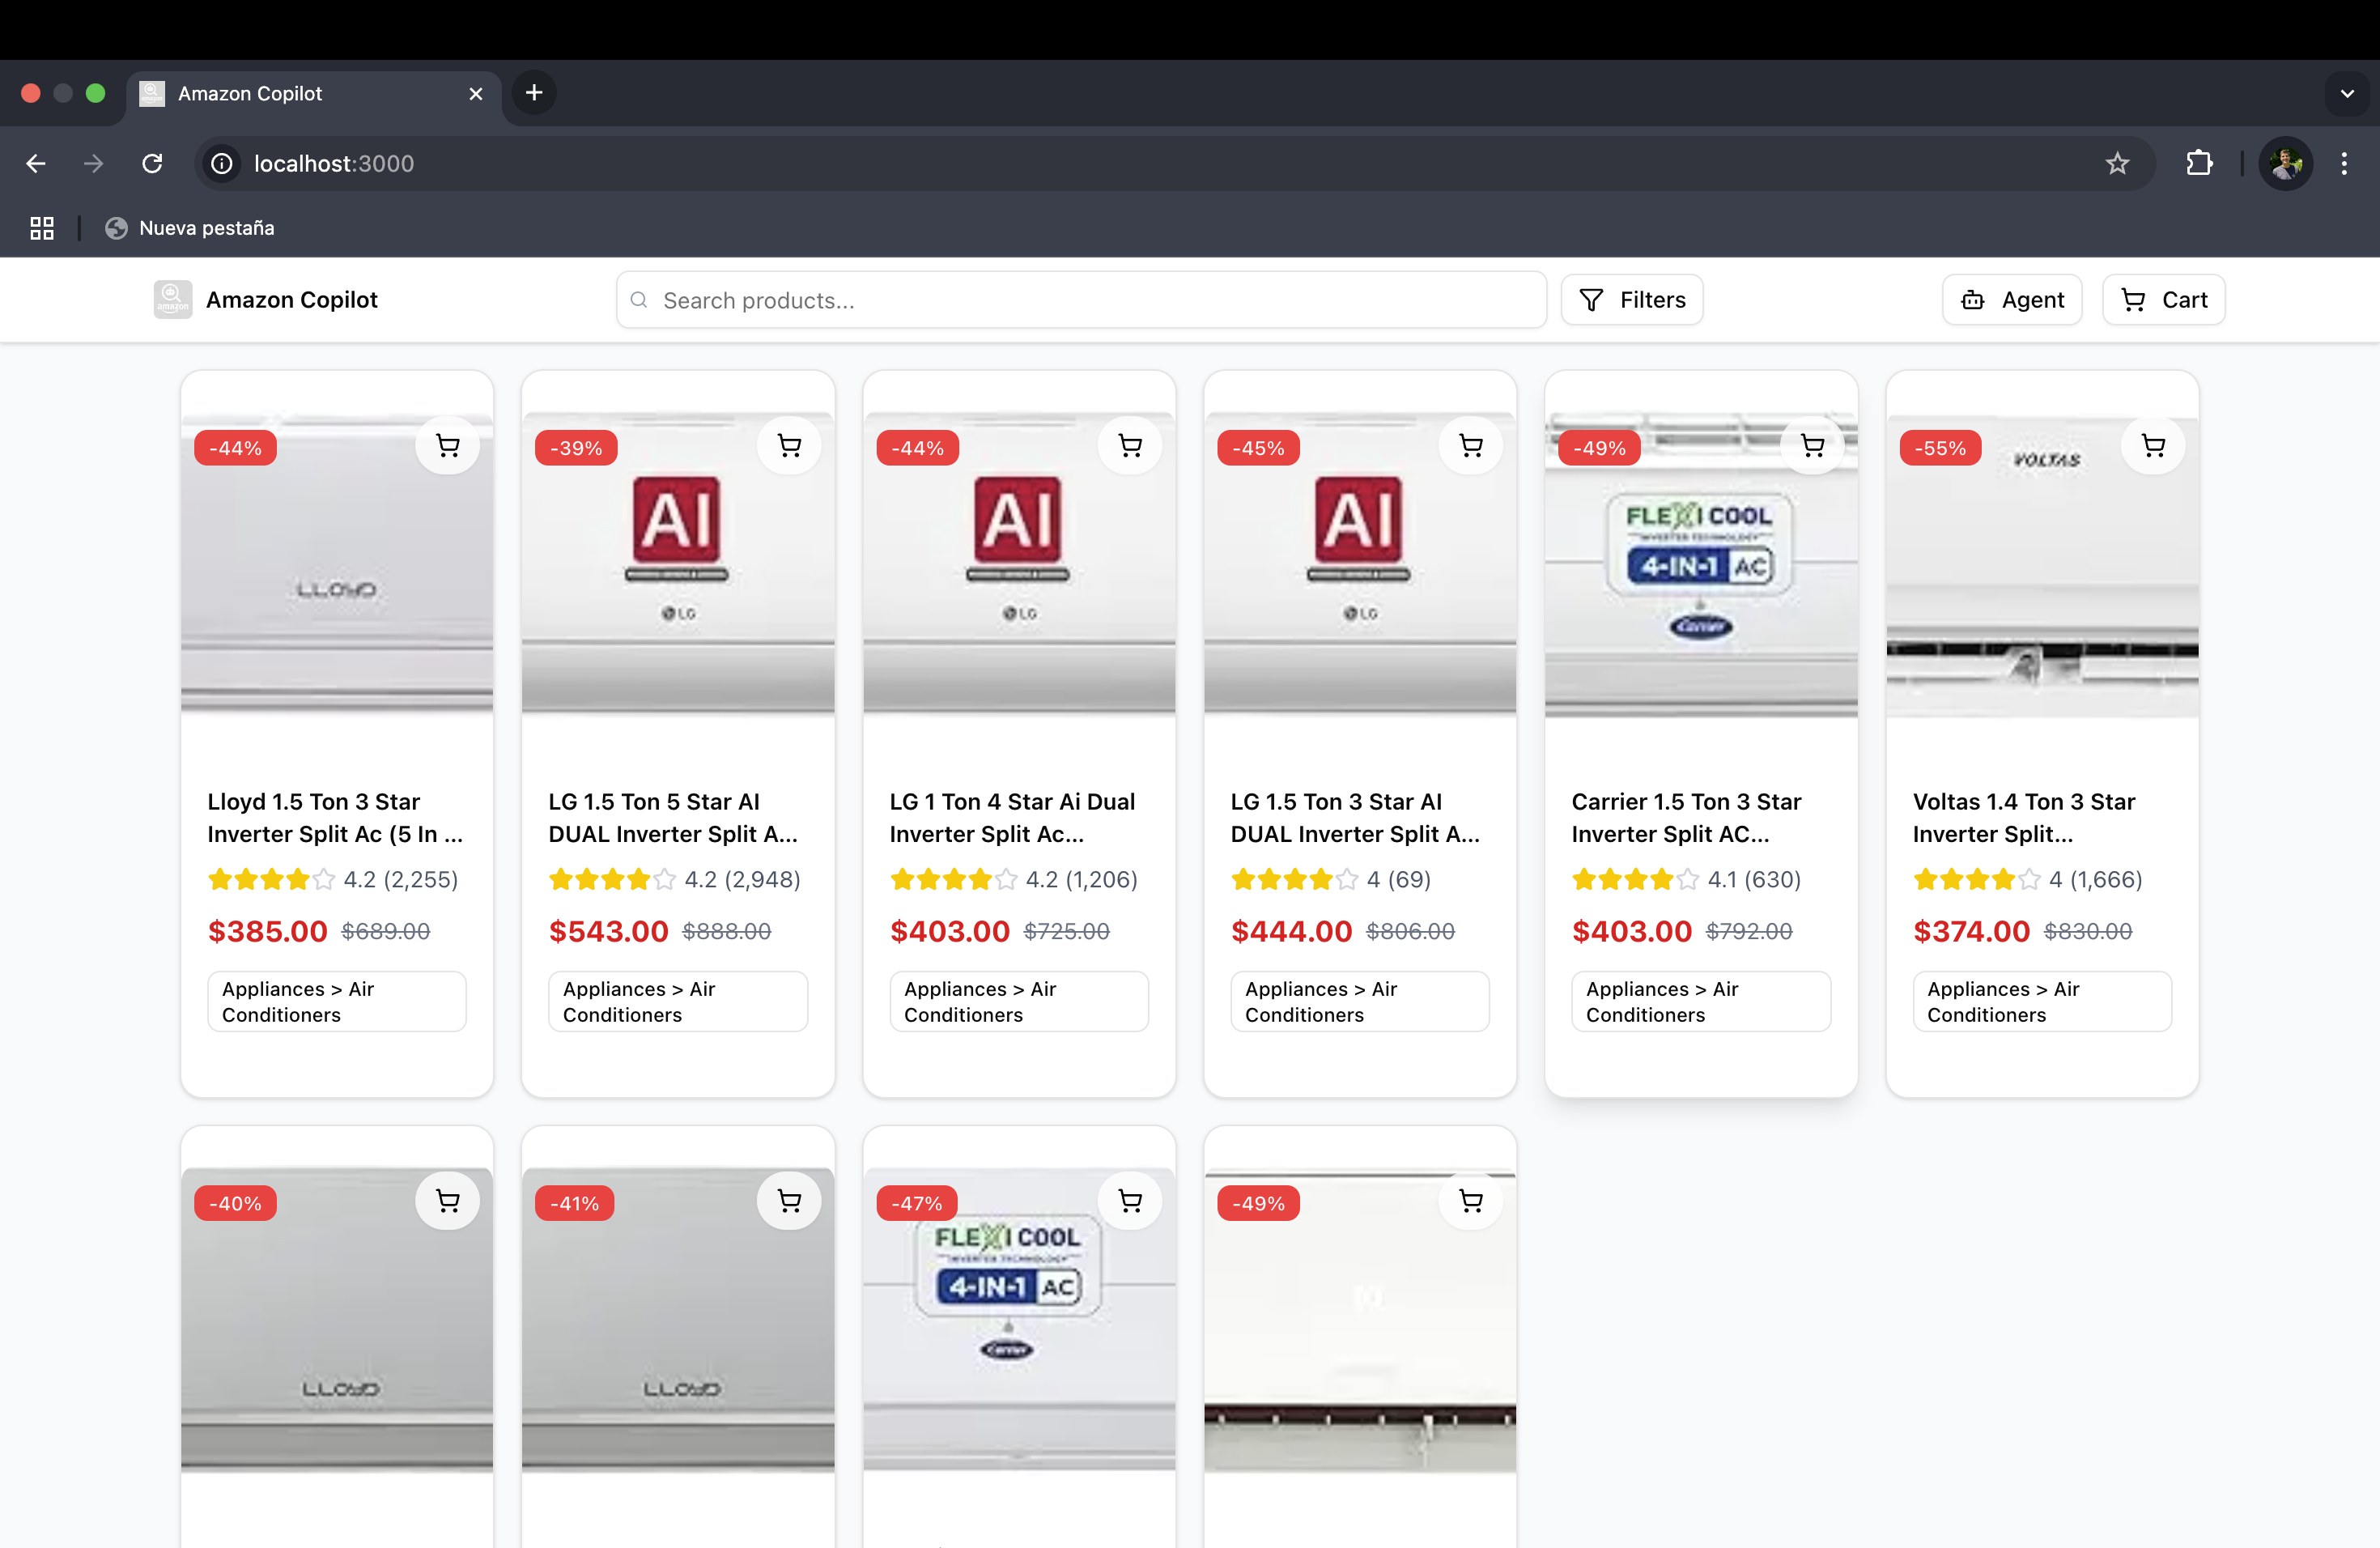
\includegraphics[width=0.8\textwidth]{home}
    \caption{Página principal - Catálogo de Productos}
\end{figure}

La interfaz incluye:
\begin{itemize}
    \item \textbf{Navbar superior}: Contiene el logo de la aplicación, barra de búsqueda y botones de navegación hacia el carrito y el asistente AI
    \item \textbf{Filtros dinámicos}: Panel lateral con categorías obtenidas dinámicamente del backend
    \item \textbf{Grid de productos}: Visualización en formato de tarjetas con información esencial (imagen, título, precio, descuento)
    \item \textbf{Paginación}: Controles para navegar entre páginas de resultados
\end{itemize}

\begin{figure}[H]
    \centering
    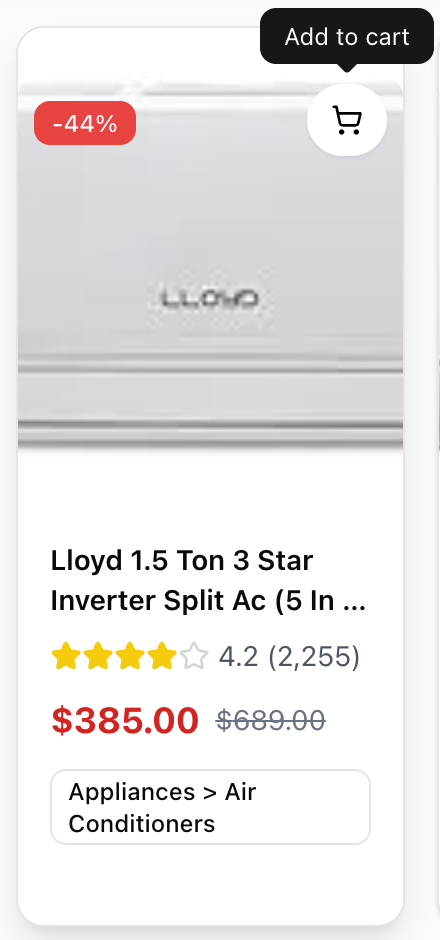
\includegraphics[width=0.45\textwidth]{product}
    \caption{Detalle de un producto en la página principal}
\end{figure}

\subsubsection{Página del Carrito}

La página del carrito (\textit{Cart}) proporciona una vista consolidada de los productos seleccionados y funcionalidades adicionales de recomendación.

\begin{figure}[H]
    \centering
    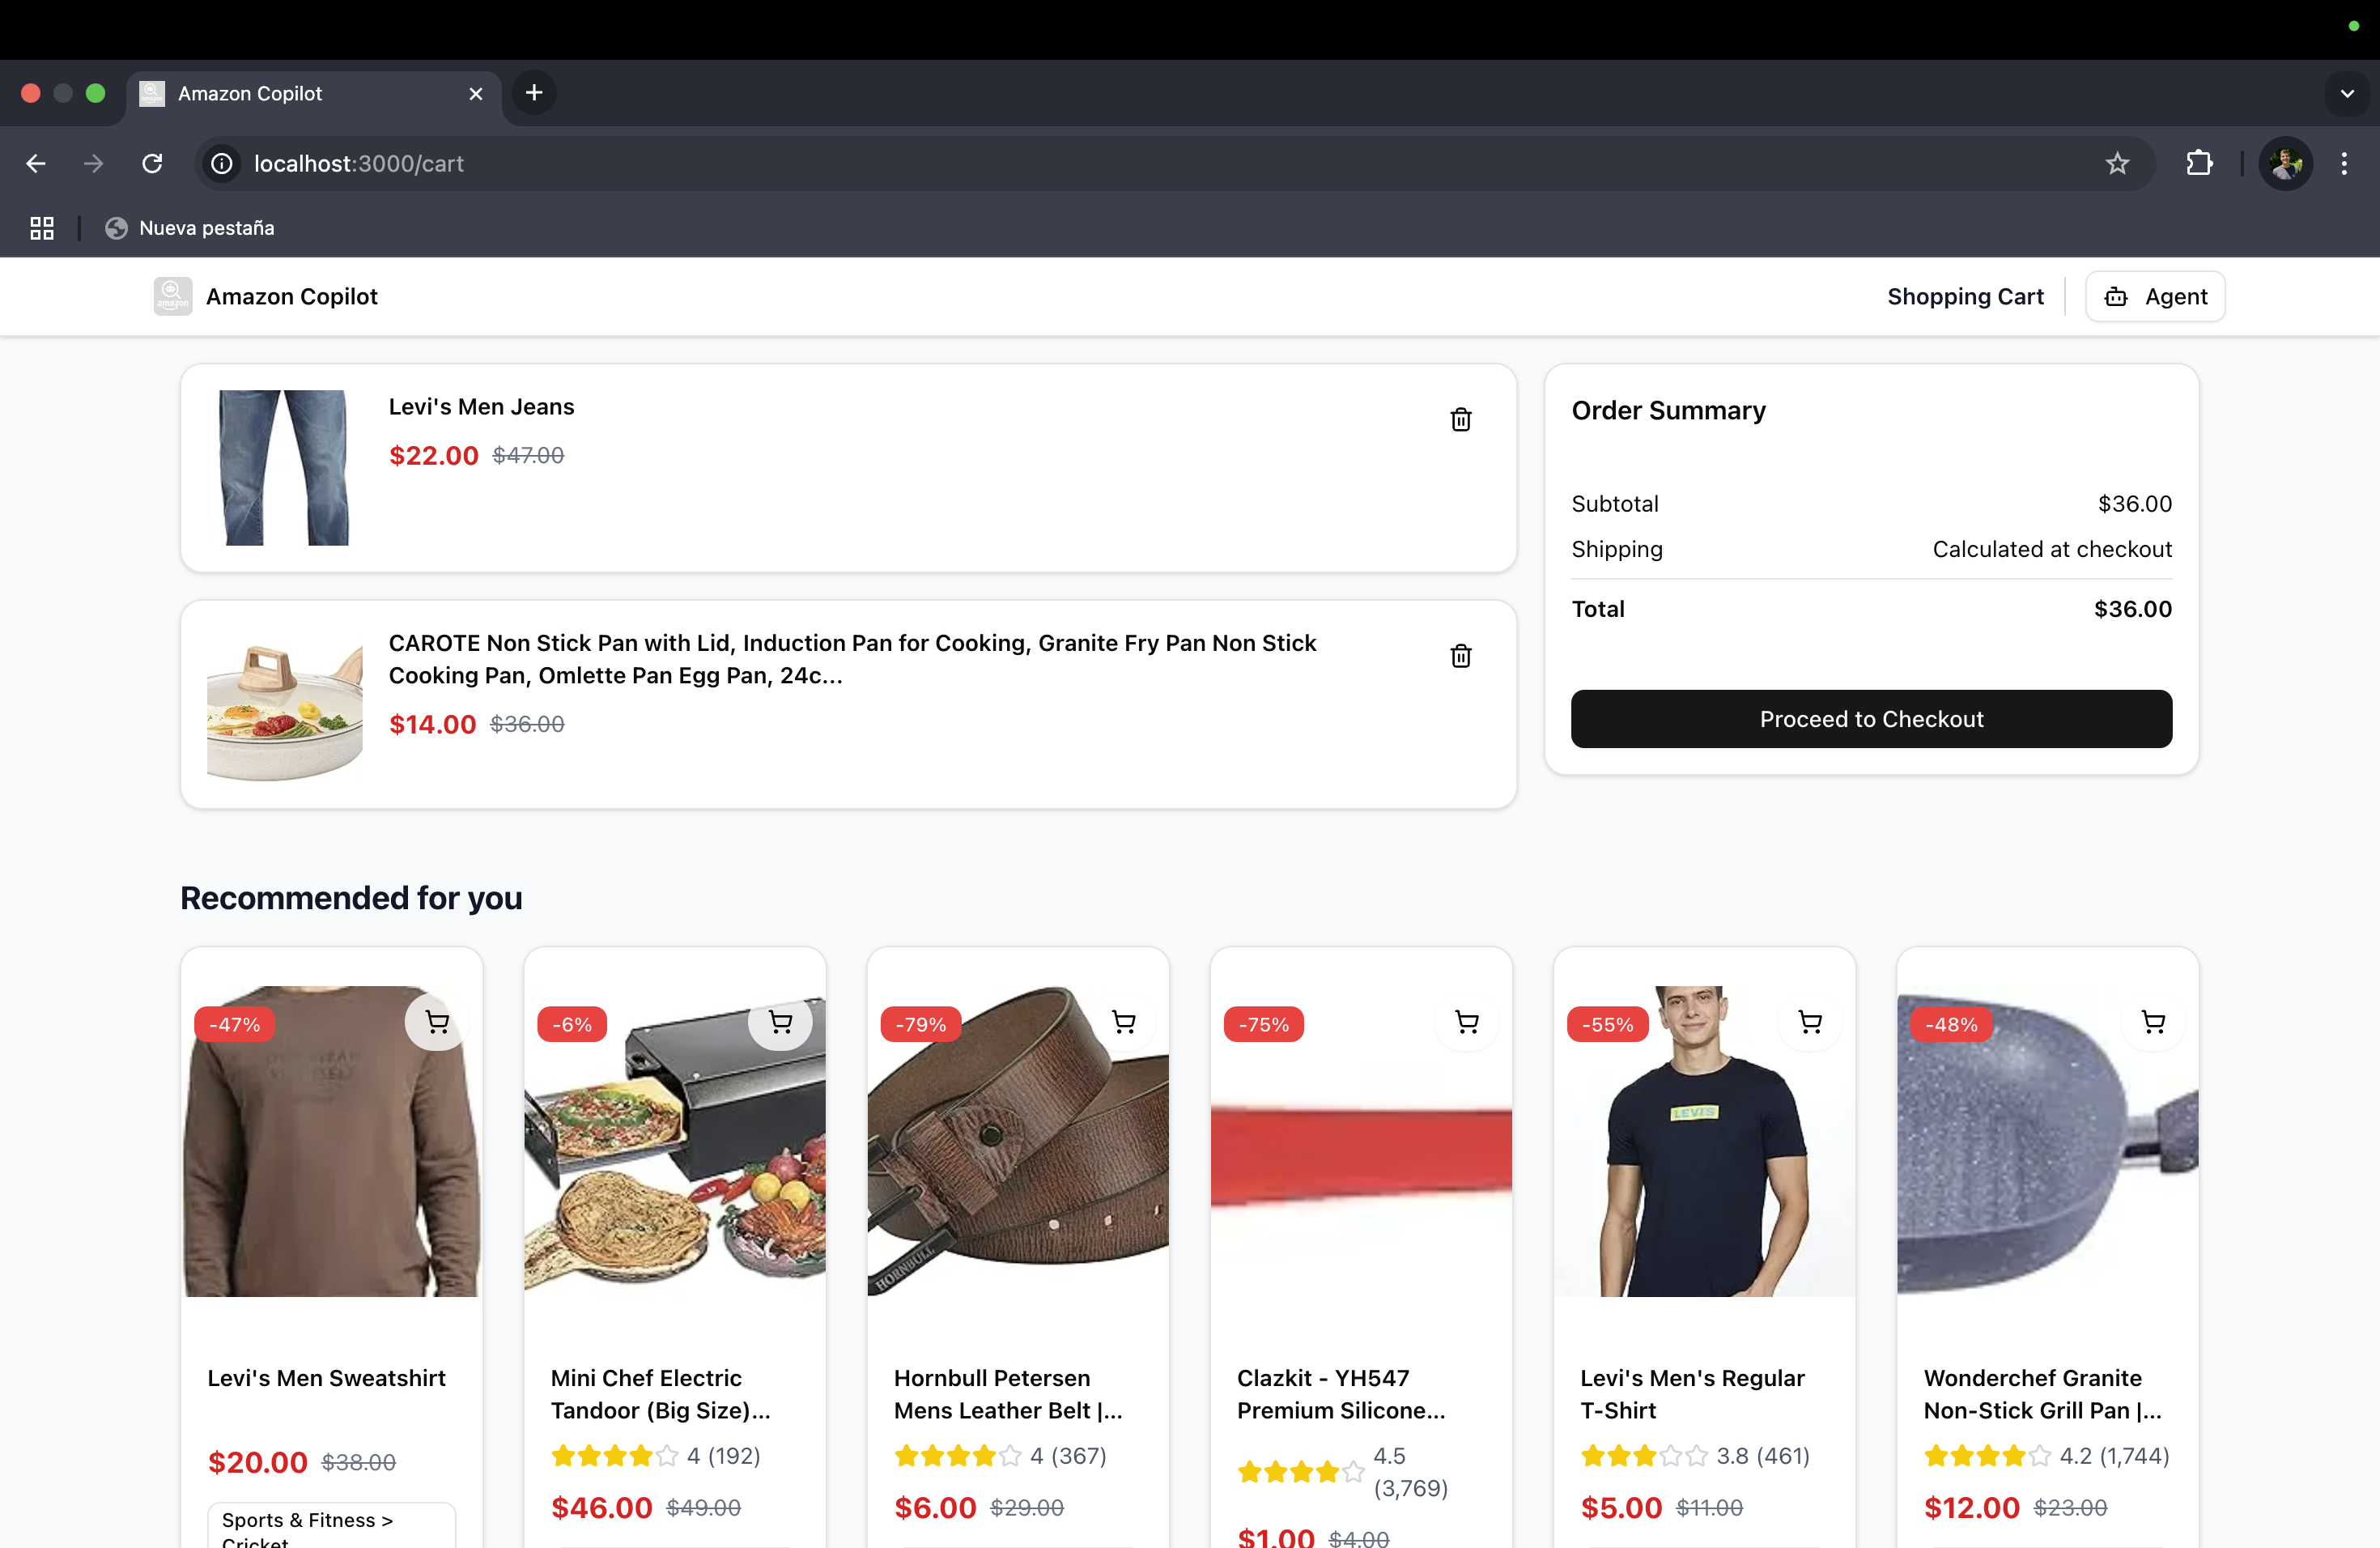
\includegraphics[width=0.8\textwidth]{cart}
    \caption{Página del carrito}
\end{figure}


Esta página se estructura en tres secciones principales:
\begin{itemize}
    \item \textbf{Lista de productos}: Muestra todos los items agregados al carrito con opciones de eliminación
    \item \textbf{Resumen de orden}: Panel lateral con el total de la compra y botón de checkout
    \item \textbf{Recomendaciones}: Sección inferior que sugiere productos relacionados basados en el contenido del carrito
\end{itemize}

\subsubsection{Página del Asistente AI}

La página del asistente (\textit{Agent}) implementa una interfaz de chat conversacional para asistir al usuario en sus consultas sobre productos.

\begin{figure}[H]
    \centering
    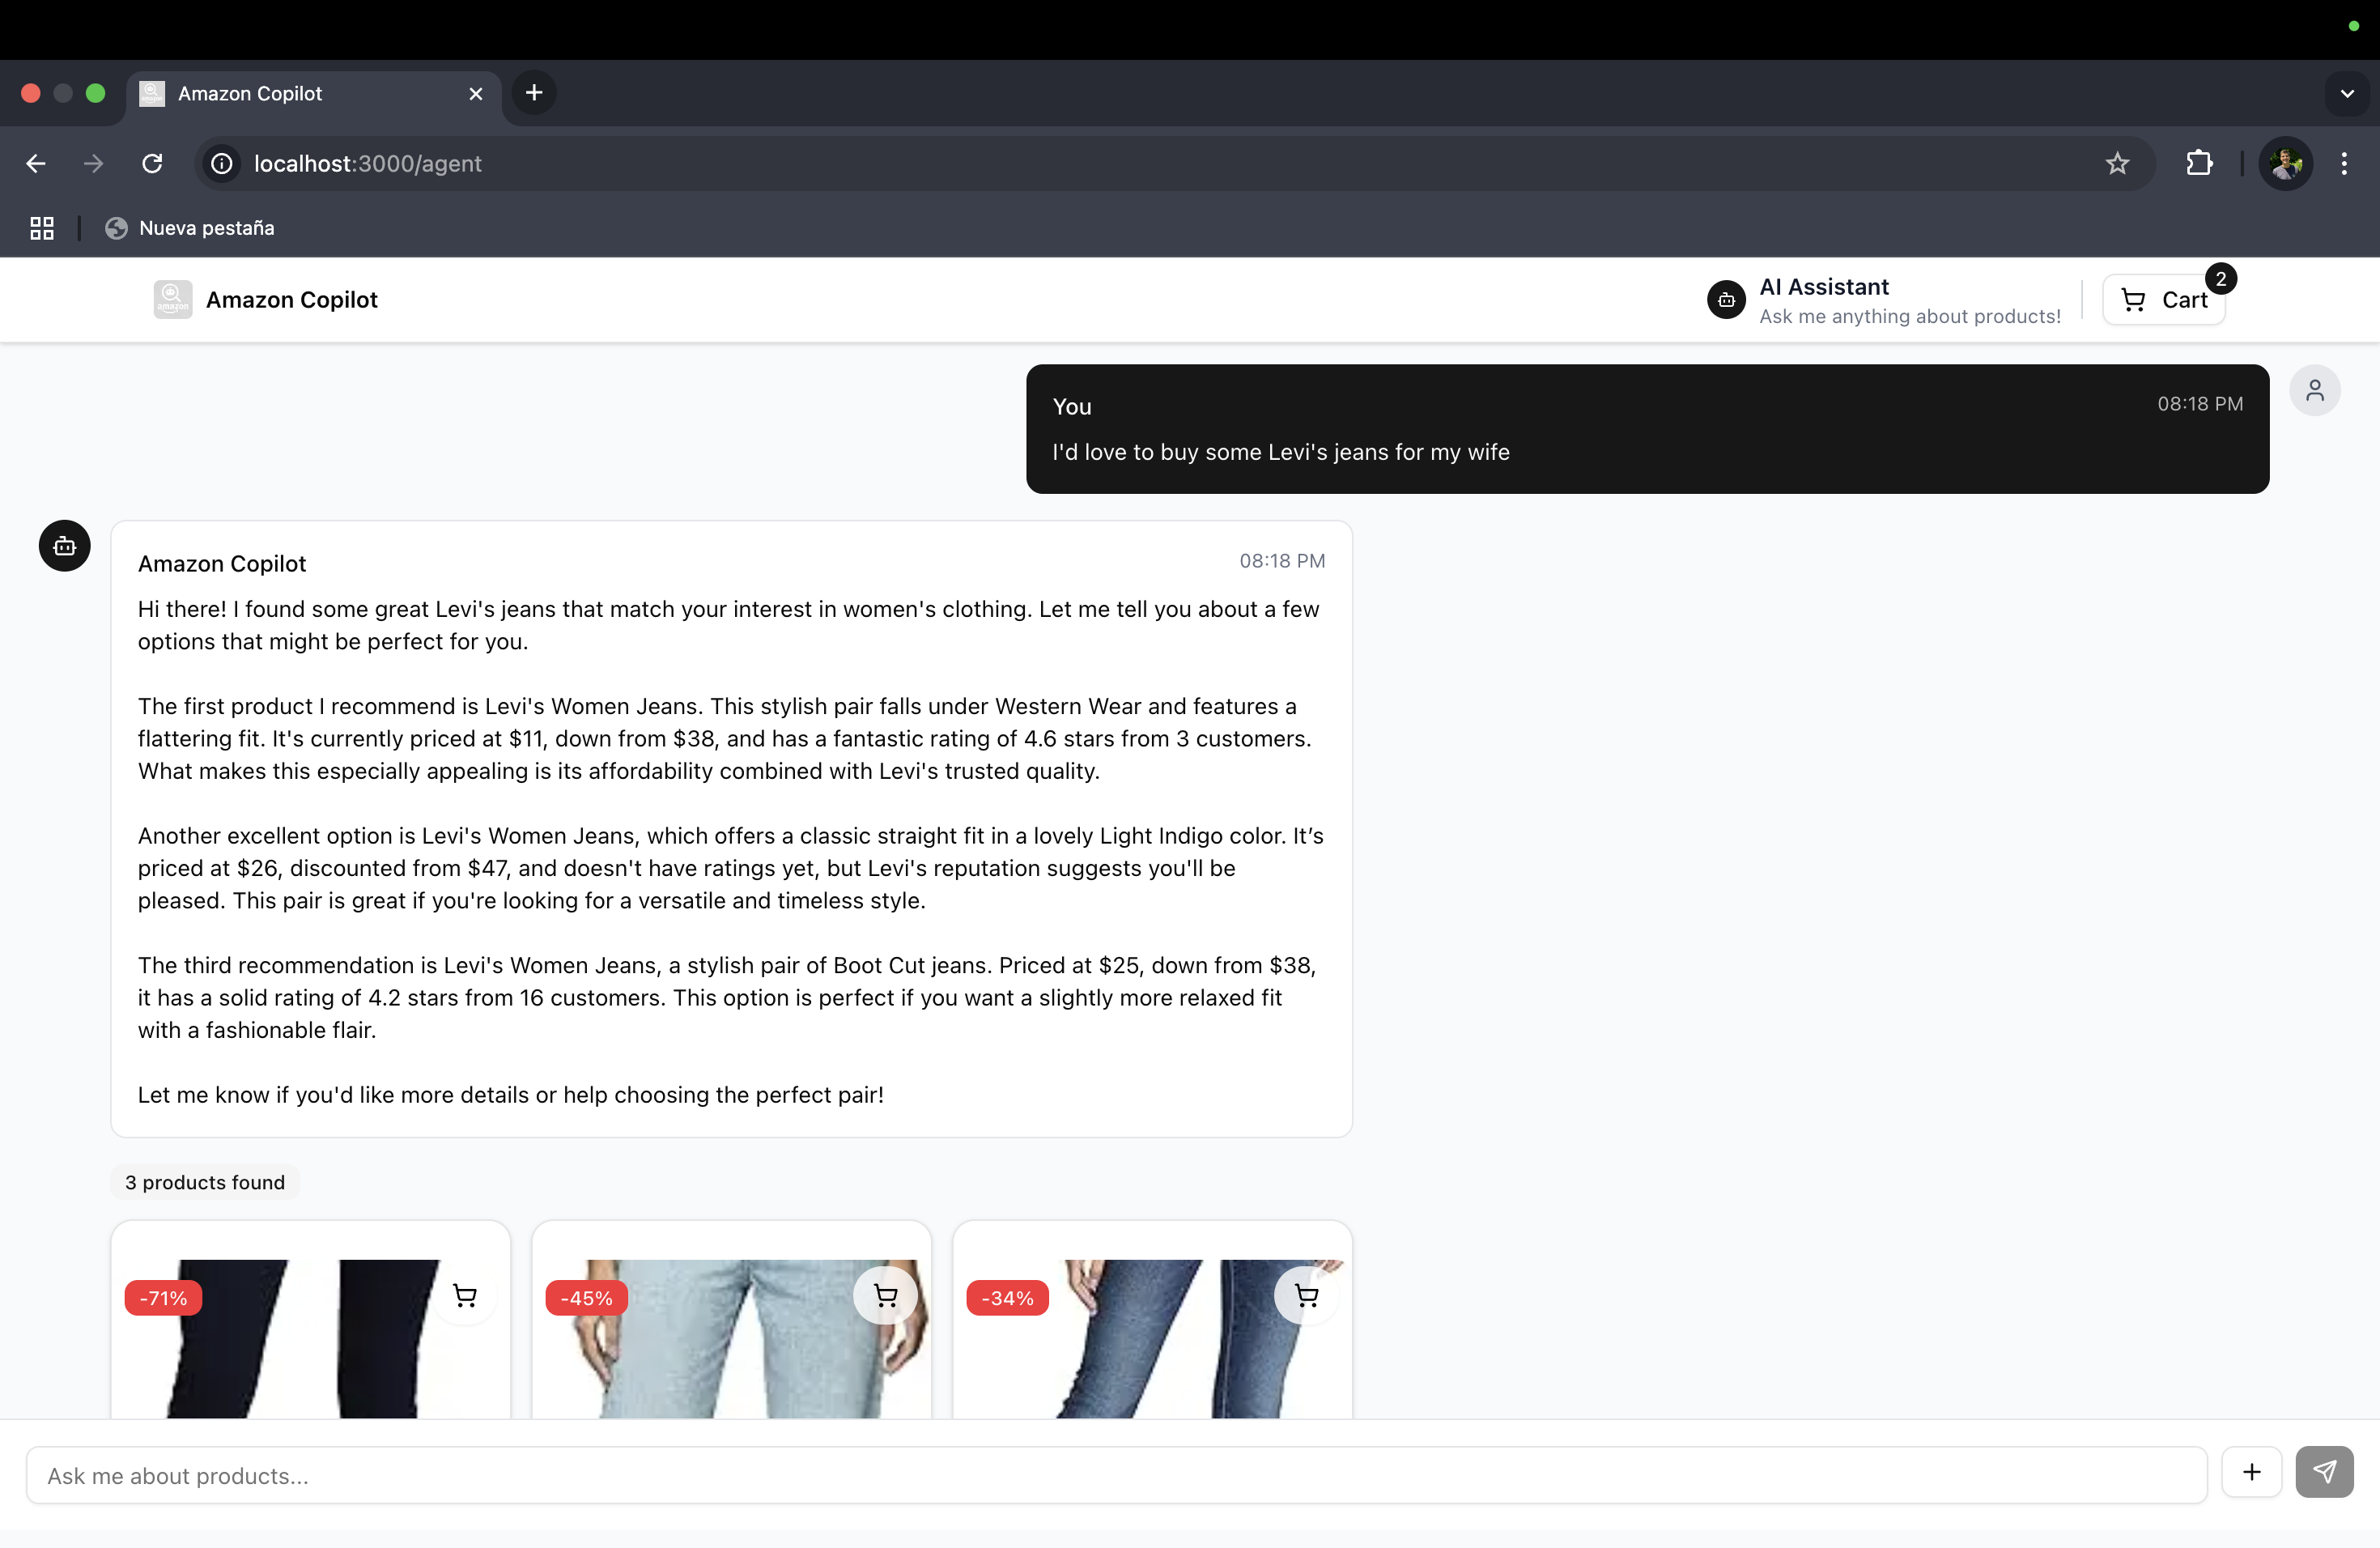
\includegraphics[width=0.8\textwidth]{agent}
    \caption{Página del asistente AI}
\end{figure}

Características principales:
\begin{itemize}
    \item \textbf{Interfaz de chat}: Diseño limpio con burbujas de mensaje diferenciadas por rol
    \item \textbf{Indicador de carga}: Feedback visual durante el procesamiento de mensajes
    \item \textbf{Productos sugeridos}: Visualización de productos recomendados por el asistente
    \item \textbf{Navegación contextual}: Enlaces directos a productos mencionados en la conversación
\end{itemize}

\subsection{Búsqueda y Filtrado Dinámico}

El sistema de búsqueda y filtrado implementa una arquitectura que optimiza tanto la experiencia del usuario como el rendimiento del backend.

\subsubsection{Filtros Dinámicos}

Los filtros de categorías se obtienen dinámicamente a través del endpoint de categorías, pero con una característica importante: las categorías disponibles se calculan en función de todos los productos existentes en la base de datos, no solo de los productos mostrados en la página actual.

\begin{figure}[H]
    \centering
    \begin{minipage}{0.45\textwidth}
        \centering
        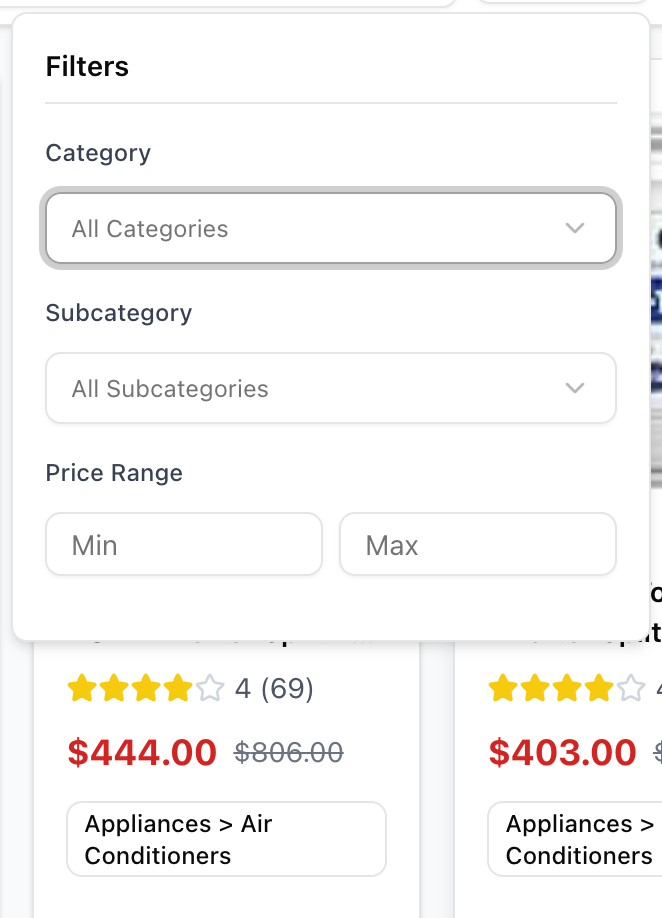
\includegraphics[width=\textwidth]{filters}
    \end{minipage}
    \hfill
    \begin{minipage}{0.45\textwidth}
        \centering
        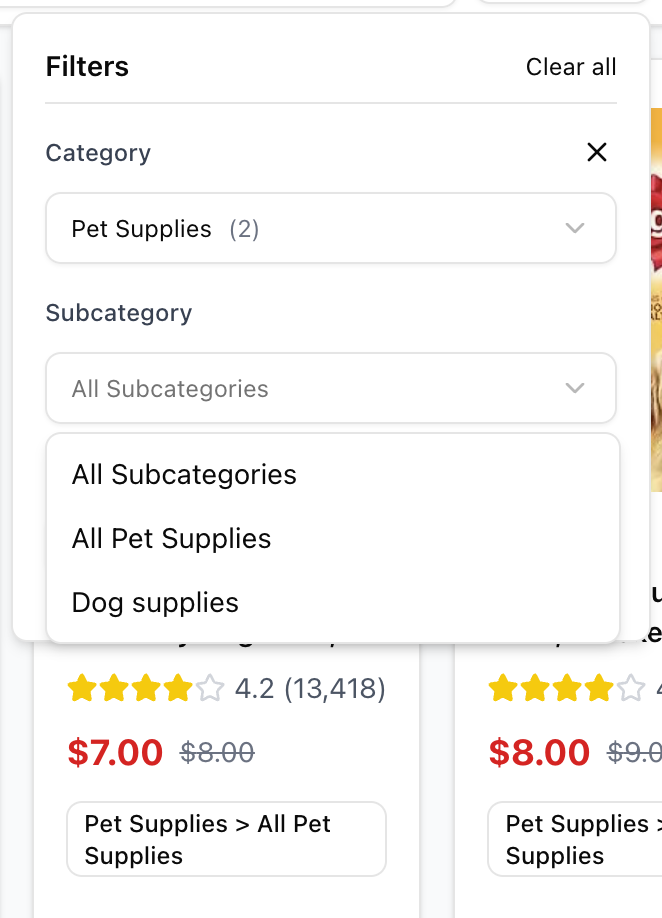
\includegraphics[width=\textwidth]{filters-2}
    \end{minipage}
    \caption{Panel de filtros}
\end{figure}

Esta implementación ofrece varias ventajas fundamentales:

\begin{itemize}
    \item \textbf{Filtrado en Backend}: Tanto los filtros como la paginación se procesan completamente en el servidor, garantizando que cada consulta se ejecute sobre la totalidad del catálogo de productos disponible
    \item \textbf{Consistencia}: Los filtros siempre reflejan la totalidad del catálogo disponible, independientemente de la página actual o los resultados mostrados
    \item \textbf{Precisión}: Evita situaciones donde un filtro no devuelve resultados debido a limitaciones de la página actual
    \item \textbf{Eficiencia}: El filtrado y paginación se realizan a nivel de base de datos, optimizando las consultas y reduciendo la transferencia de datos innecesaria
    \item \textbf{Escalabilidad}: La arquitectura permite manejar catálogos de gran tamaño sin impactar el rendimiento del frontend
\end{itemize}

El flujo de procesamiento garantiza que cada búsqueda, filtro o cambio de página resulte en una nueva consulta al backend que opera sobre el conjunto completo de productos, asegurando resultados precisos y consistentes en todo momento.

\subsubsection{Query Parameters y Reactividad}

La aplicación utiliza query parameters para triggerear nuevas consultas, implementando un sistema reactivo que actualiza automáticamente los resultados cuando el usuario modifica los filtros o la búsqueda.

\begin{figure}[H]
    \centering
    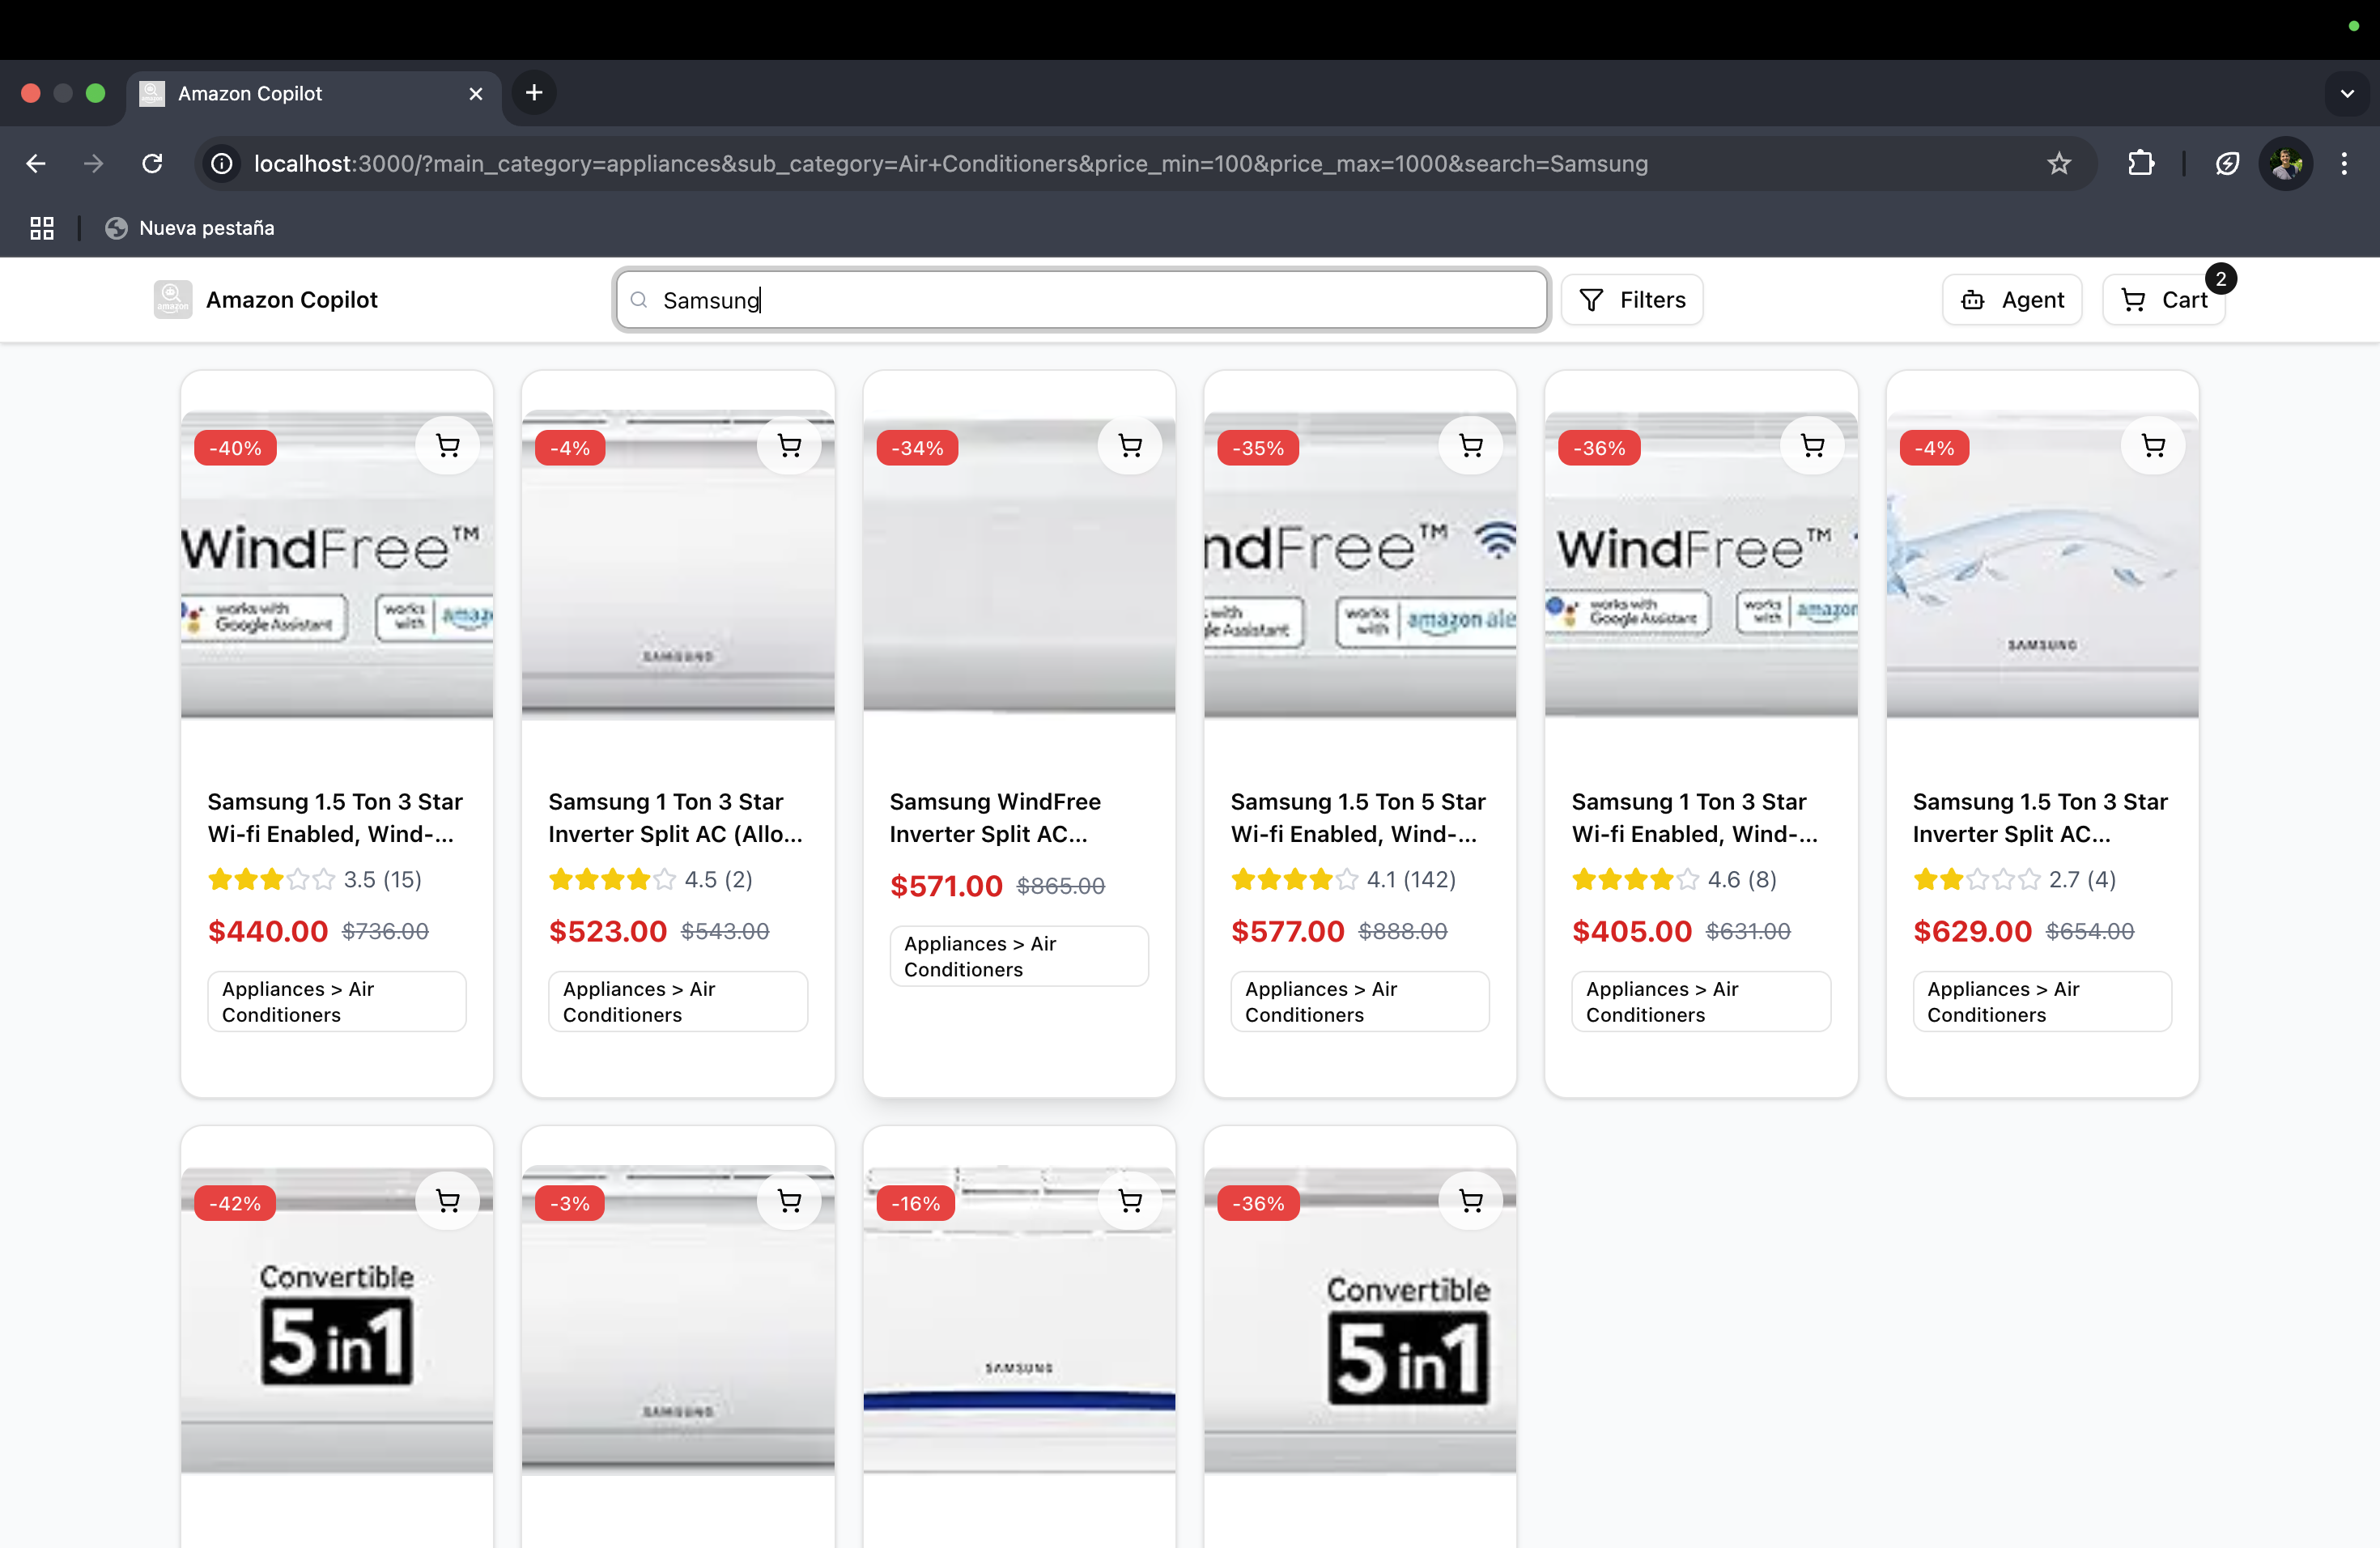
\includegraphics[width=0.8\textwidth]{query-parameters}
    \caption{URL con query parameters}
\end{figure}

El flujo de actualización funciona de la siguiente manera:
\begin{enumerate}
    \item El usuario modifica un filtro o realiza una búsqueda
    \item Los query parameters se actualizan en la URL
    \item Next.js detecta el cambio y re-renderiza la página
    \item Se ejecuta una nueva consulta al backend con los parámetros actualizados
    \item Los resultados se muestran al usuario
\end{enumerate}

Esta implementación ofrece ventajas adicionales:
\begin{itemize}
    \item \textbf{URLs compartibles}: Los usuarios pueden compartir resultados específicos simplemente copiando el enlace, ya que todos los parámetros de búsqueda y filtrado están codificados en la URL
    \item \textbf{Reproducibilidad}: Cualquier usuario puede reproducir exactamente los mismos resultados accediendo al enlace compartido
    \item \textbf{Bookmarking}: Los usuarios pueden guardar búsquedas específicas como favoritos en su navegador
\end{itemize}

\subsection{Arquitectura de Server Components y Suspense}

La aplicación aprovecha las capacidades avanzadas de Next.js 14, específicamente los Server Components y Suspense, para optimizar el rendimiento y la experiencia de usuario.

\subsubsection{Server Components}

Los Server Components permiten que la ejecución de queries comience desde el momento en que el navegador realiza la consulta al servidor web, no después de que se cargue el JavaScript en el cliente.

% [INSERTAR IMAGEN: Diagrama mostrando el flujo de Server Components vs Client Components]

Beneficios de esta arquitectura:
\begin{itemize}
    \item \textbf{Inicio temprano}: Las consultas se ejecutan en paralelo con la generación del HTML
    \item \textbf{Mejor SEO}: El contenido se renderiza en el servidor, mejorando la indexación
    \item \textbf{Menor JavaScript}: Reduce la cantidad de código que debe descargarse al cliente
    \item \textbf{Mejor rendimiento inicial}: La página se muestra más rápido al usuario
\end{itemize}

Además, la aplicación aprovecha los \textbf{Server Actions} de Next.js para operaciones que requieren interacción del servidor, como el envío de mensajes al asistente AI y la generación de recomendaciones de productos. Los Server Actions permiten ejecutar código del servidor directamente desde componentes del cliente, proporcionando una experiencia fluida sin necesidad de crear endpoints API separados.

\subsubsection{Suspense y Estados de Carga}

El componente Suspense se utiliza para proporcionar una experiencia de usuario fluida durante la carga de datos, implementando loading states que se muestran mientras se stremea el HTML con los datos.

\begin{figure}[H]
    \centering
    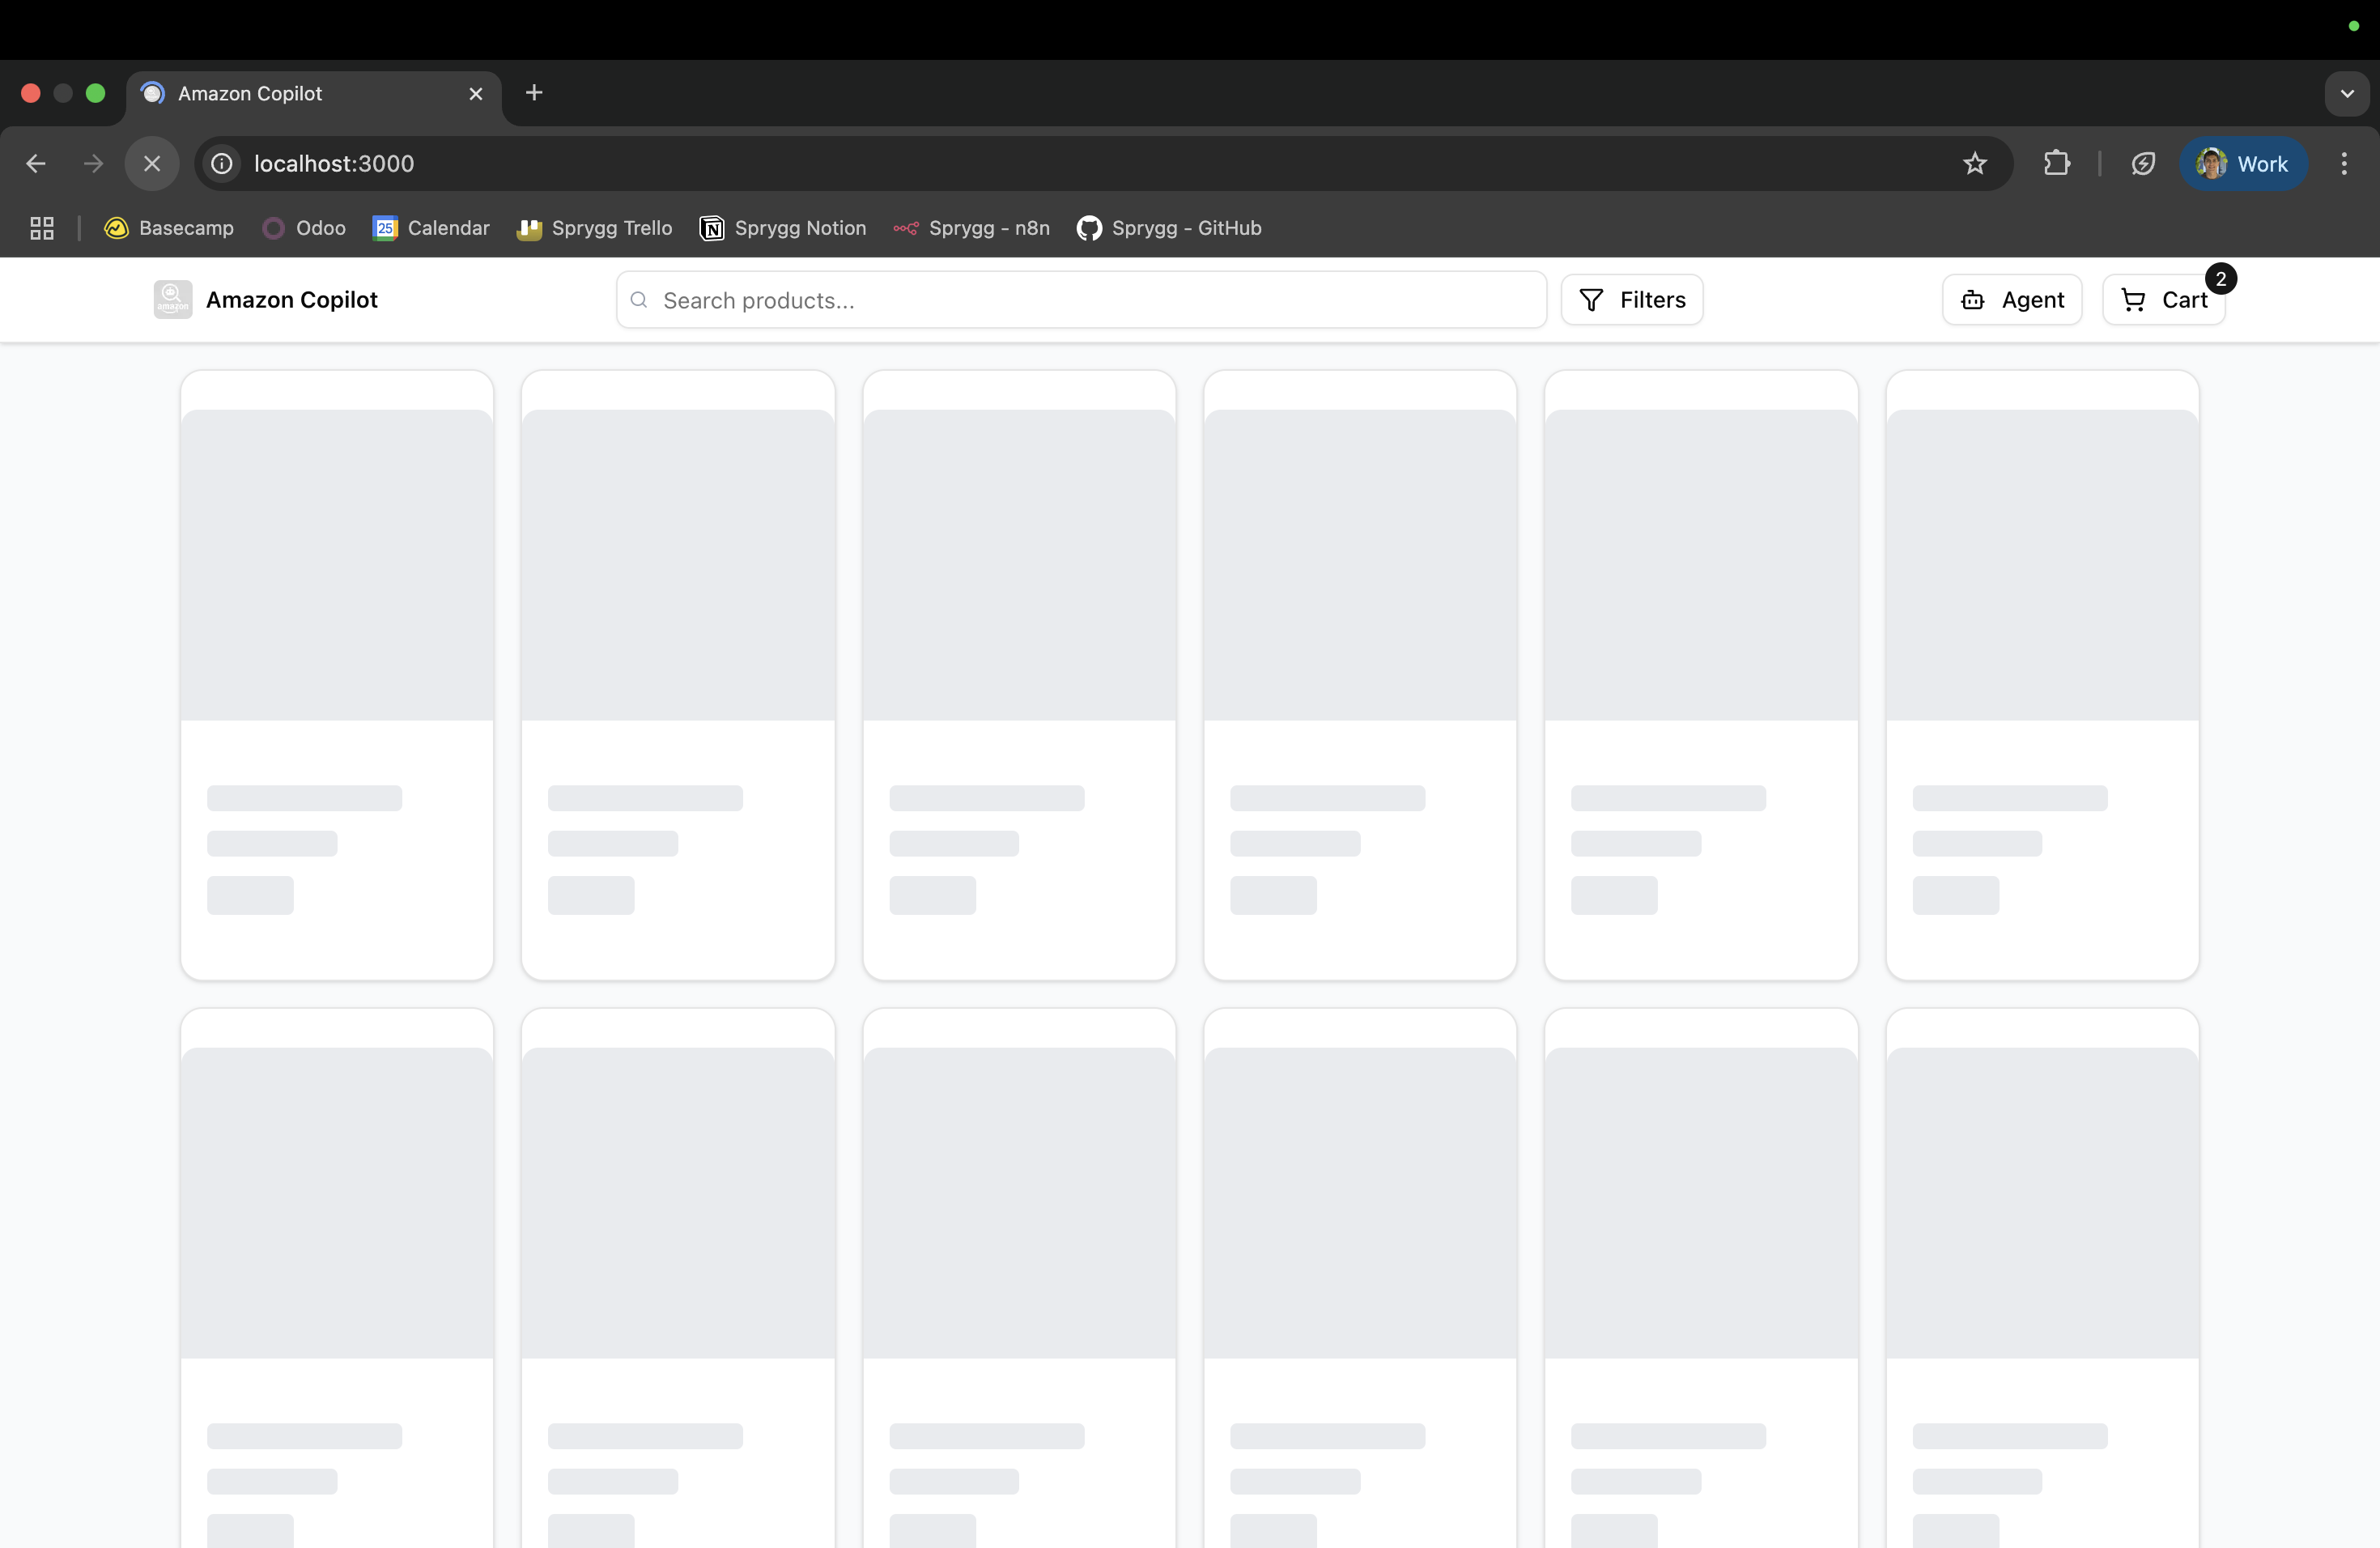
\includegraphics[width=0.8\textwidth]{skeleton}
    \caption{Estado de carga con Suspense}
\end{figure}


La implementación incluye:
\begin{itemize}
    \item \textbf{Skeleton loading}: Placeholders animados que simulan la estructura del contenido
    \item \textbf{Streaming progresivo}: Los datos se envían al cliente tan pronto como están disponibles
    \item \textbf{Transiciones suaves}: Los estados de carga se reemplazan sin interrupciones visuales
\end{itemize}

\subsection{Gestión de Estado con Contextos}

Para el carrito y el chatbot, se implementó un sistema de gestión de estado basado en contextos de React, combinado con almacenamiento local en el navegador.

\subsubsection{Contexto del Carrito}

El contexto del carrito maneja el estado de los productos seleccionados, almacenándolos en localStorage para persistencia entre sesiones.

Características principales:
\begin{itemize}
    \item \textbf{Persistencia local}: Los productos se mantienen entre recargas de página
    \item \textbf{Sincronización automática}: Cambios en el carrito se reflejan inmediatamente en toda la aplicación
    \item \textbf{Recomendaciones dinámicas}: Los productos del carrito se utilizan para generar recomendaciones personalizadas
\end{itemize}

\subsubsection{Contexto de Conversación}

El contexto de conversación gestiona el estado del chat con el asistente AI, implementando una estrategia híbrida de almacenamiento.

La implementación distingue entre dos tipos de datos:
\begin{itemize}
    \item \textbf{Mensajes}: Se almacenan en localStorage únicamente para su visualización en la interfaz
    \item \textbf{Identificador de conversación}: Se mantiene para preservar el contexto de la conversación en el backend
\end{itemize}

Esta separación permite:
\begin{itemize}
    \item \textbf{Contexto persistente}: El asistente mantiene memoria de mensajes anteriores
    \item \textbf{Experiencia fluida}: Los mensajes se muestran inmediatamente sin necesidad de recargar
    \item \textbf{Eficiencia de almacenamiento}: No se requiere una base de datos adicional para el estado
\end{itemize}

Esta arquitectura es especialmente adecuada para prototipos y aplicaciones de demostración, donde la simplicidad y velocidad de desarrollo son prioritarias sobre la persistencia a largo plazo de datos de estado.
